\subsection{UC-4}

\begin{figure}[H]
    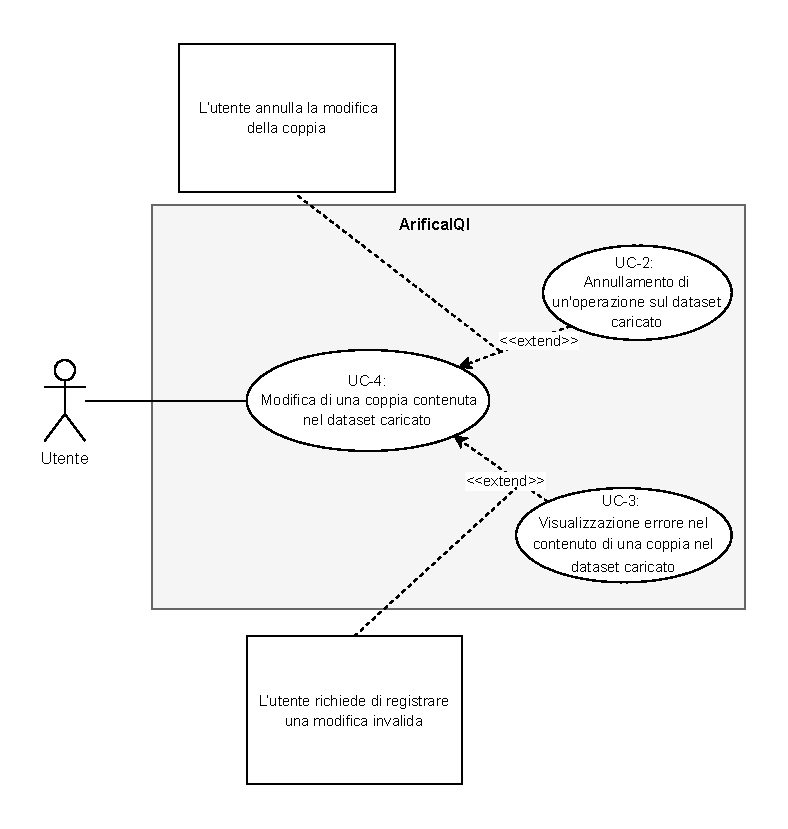
\includegraphics[scale=0.8]{Sezioni/UseCase/Immagini/UC-4.pdf}
    \caption{Diagramma UC-4.}
\end{figure}

\begin{usecase}{UC-4}{Modifica di una coppia contenuta nel dataset caricato}
    
    \req{\hyperref[item:RU-1]{RU-1}} 

    \pre{
        \item Il sistema è attivo e funzionante
        \item La coppia da modificare è contenuta nel dataset caricato
    }

    \post{
        \item La coppia da modificare nel dataset caricato viene aggiornata
    }
    
    \actor{Utente}

    \subactors{}

    \trigger{L'utente deve modificare una coppia contenuta nel dataset caricato}
    
    \inc{}

    \base{}

    \scenario{
        \item L'utente richiede la modifica di una coppia del dataset caricato
        \item L'utente modifica il contenuto della coppia
        \item L'utente conferma la modifica della coppia
        \item La coppia viene aggiornata nel dataset caricato

    }

    \subscenario{
        \item[2.1] \textbf{L'utente annulla la modifica della coppia} 
        \begin{itemize}
            \item[a.] \hyperref[subsec:UC-2]{UC-2}
        \end{itemize}
        \item[3.1] \textbf{L'utente richiede di registrare una modifica invalida}
        \begin{itemize}
            \item[a.] \hyperref[subsec:UC-3]{UC-3}
        \end{itemize}
    }
\end{usecase}
